\subsection{Database}
Since the web app requires a database to store information about users, questions, sessions, subjects and more. A set of files were created to get, insert and update information. The database is designed around features needed for the application, and it was also created for scalability in mind with for example the possibility to add other OAuth/openid connect possibilities in the future. There are five scripts associated with the database, where get, insert and update functions has been separated into their own scripts. One script is connecting the get, insert and update scripts making it easier to import and use the database functions in other scripts. There is also a script that will run every time the server starts. This script will make sure that every table is created and have the correct column names. It is also the script that will insert default values such as question types and the anonymous user.
\begin{figure}[H]
    \centering
    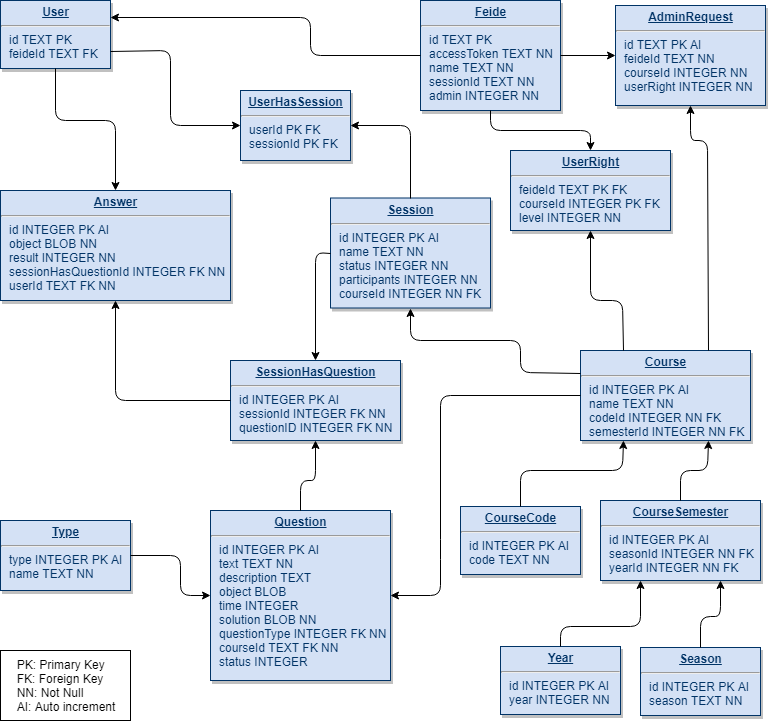
\includegraphics[width=\linewidth]{diagrammer/databaseSchema.png}
    \caption{This is the database schema used for Interaktiv Undervisning}
    \label{fig:dbSchema}
\end{figure}
The table "User" will have the anonymous user with user id 1, so when an anonymous user answers a question that answer will be linked to that user, no matter who answered. Also since feide information is in its own table, this makes it easy to add more types of login services, e.g., facebook, google, and more. When an admin adds a question to a session, it will be linked in its own table called QuestionHasSession. This is to ensure that a question can be linked to more than one session or multiple times in the same session. The answers are also linked to the QuestionHasSession table making sure that the answers show to admins are only for that question in that session and not the total answers statistics for that question. Sessions are also linked to a subject where the primary key is a combination between the course code and course semester, making sure that an admin gets the sessions for a specific course and year. Questions are linked to the course id, but admins does have the option to copy questions from one course to another in the question dashboard.